\section{Part-of-Speech Tagging with CRF}

\subsection*{Goal}

Classify the grammatical categories of each word, e.g. noun, verb, etc.
$p(t\mid w) = \frac{\exp(\text{score}(t,w))}{Z(w)}$ for a tagging sequence $t$ and a sentence $w$ of length $N$.

\subsection*{Conditional Random Field}

Idea: use additively decomposable score function. $\text{score}(w,t) = \sum_{n=1}^{N} \text{score}(<t_{n-1}, t_n>, w)$.

The normalizer can be computed by DP (semiring: $(R^+ \cup \{+\infty\}, +, \times, 0, 1)$):
\begin{center}
    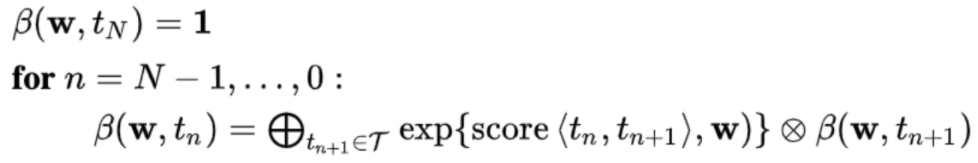
\includegraphics[width=.23\textwidth]{img/CRF-normalizer.png}
\end{center}
and $Z(w) = \beta(w, t_0)$.

\subsection*{Decoding the best POS tagging}

Equivalent to compute the maximum-score path. Use Viterbi (semiring: $([0,1], \max, \times, 0, 1)$).

\subsection*{Semiring}

Def: (1) addition should be commutative, (2) multiplication should distribute over addition, (3) addition and multiplication have identities, and (4) identity of addition should be an annihilator for multiplication.
\begin{center}
    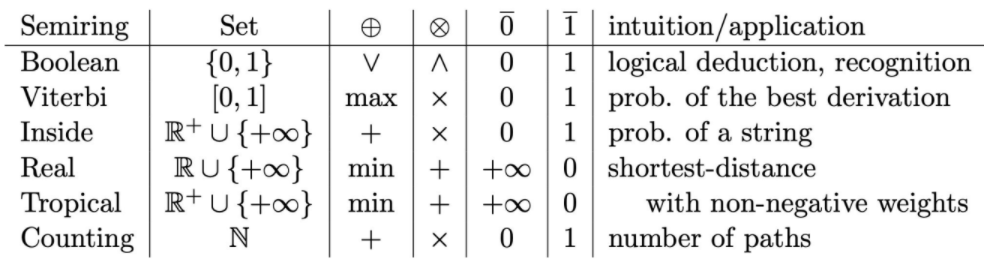
\includegraphics[width=\columnwidth]{img/semiring.png}
\end{center}

\subsection*{Structured Perceptron}

The MLE loss for CRF is a softmax, so we add a temperature variable and take it to infinity, the loss becomes $\sum_i (\text{score}(t^i, w^i) - \max_{t^\prime} \text{score}(t^\prime, w^i))$. This is called structured perceptron.